\section{Introduction}
\label{sec:intro}

A connected vehicle that receives another agent's detections must place them in its own frame, and the only thing it has for that is the sender's self-reported pose. GNSS and odometry are wrong by decimetres in the open and by metres in urban canyons, and a pose error displaces the sender's whole box set rigidly. Every shared object becomes a duplicate at the wrong place, and every unshared one a false positive. Fig.~\ref{fig:problem} illustrates the effect and Fig.~\ref{fig:teaser} shows its size.

\begin{figure}[t]
  \centering
  % Fig: why an uncorrected pose error breaks late fusion. Problem only, no AlignFormer.
\resizebox{\linewidth}{!}{%
\begin{tikzpicture}[
  >=Latex, node distance=0.34cm,
  blk/.style={draw=black!60, line width=0.5pt, rounded corners=1.5pt, fill=white, inner sep=3pt, align=center,
              font=\footnotesize, minimum height=1.0cm, text width=1.75cm},
  io/.style={blk, fill=black!6, draw=black!40, text width=1.6cm},
  arr/.style={->, line width=0.6pt, black!70}]
  \node[io, fill=orange!12, draw=orange!70!black] (cavbox) {CAV boxes $\mathcal{Q}$\\+ reported pose};
  \node[blk, right=of cavbox] (proj) {project into\\ego frame};
  \node[io, right=of proj, fill=orange!12, draw=orange!70!black] (misq) {$\mathcal{Q}$, received\\(misaligned)};
  \node[io, below=0.85cm of cavbox, fill=green!10, draw=green!50!black] (ego) {ego boxes\\$\mathcal{P}$};
  \node[blk, right=of misq, below=0.42cm of misq, fill=black!6] (fuse) {late fusion\\(NMS)};
  \node[io, right=of fuse, fill=red!8, draw=red!60!black, text width=1.75cm] (out) {duplicate /\\false positive};
  \draw[arr] (cavbox) -- (proj);
  \draw[arr] (proj) -- (misq);
  \draw[arr] (misq) -- (fuse);
  \draw[arr] (ego.east) -| (fuse.west);
  \draw[arr] (fuse) -- (out);
\end{tikzpicture}}

  \caption{\textbf{The problem.} A pose error in the CAV's self-reported position displaces its whole detected box set rigidly, turning shared detections into duplicates and false positives.}
  \label{fig:problem}
\end{figure} On \opvv, plain late fusion scores 0.896 \ap{0.7} with exact poses and 0.316 with \SI{0.4}{m} of Gaussian pose noise. On \vxreal the same step is 0.422 to 0.216. Without a correction, the cooperative detector is worse than the ego alone.

\begin{figure}[t]
  \centering
  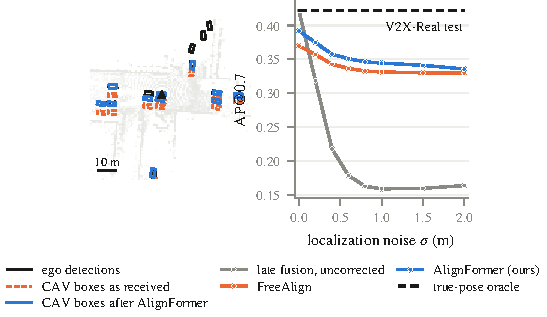
\includegraphics[width=\linewidth]{figures/teaser.pdf}
  \caption{\textbf{Localization error and what remains of it.} Left: a \vxreal frame (val) whose CAV reports its pose with $\sigma=\SI{2}{m}$ noise. Its boxes arrive \SI{4.4}{m} from where the objects are, beside the ego's own detections of the same cars, and late fusion keeps both. \paper puts them \SI{0.11}{m} from the truth from the boxes alone. Right: \ap{0.7} on \vxreal test (2,172 frames, mean of 5 noise seeds, standard errors below the marker size) against the localization noise $\sigma$, whose yaw component is $\sigma$ degrees. Uncorrected late fusion loses 60\% of its clean AP by $\sigma=\SI{1}{m}$. \freealign~\cite{lei2024freealign} recovers most of it, and \paper is above \freealign at every $\sigma$, including $\sigma=0$.}
  \label{fig:teaser}
\end{figure}

Two families of remedies exist. Intermediate-fusion methods~\cite{vadivelu2020learning,lu2023coalign,hong2024mrcnet} correct the pose inside a shared bird's-eye-view feature pipeline. They need megabytes per frame and a jointly trained backbone on every agent. Late-fusion methods work on detected boxes and are therefore cheap and detector-agnostic. The strongest of them, \freealign~\cite{lei2024freealign}, needs no localization at all. It builds a graph per agent whose nodes are boxes and whose edges are relative distances, which are invariant to the sender's pose, matches common subgraphs, and fits the pose by RANSAC over the matched nodes. In our measurements \freealign's correction is flat across the whole noise range, exactly as its paper claims.

\freealign also has two structural weaknesses, and this paper is built on them. First, a relative-distance graph on fewer than three shared objects is degenerate, so \freealign declines the pair. On \opvv it abstains on 84\% of the pairs sharing one or two objects, and on \vxreal those pairs are a quarter of all frames. A method that learns the association from the boxes' absolute geometry, including heading, can answer them. A single matched object with a heading already determines an $\SE$ transform. Second, \freealign's pose is only as good as its hard matches. An exact fit over a wrong correspondence is exactly wrong, and 2.6\% of its corrections on \opvv are off by more than \SI{3}{m}, three times our rate. A soft, learned estimator has the opposite failure. Its answer is a weighted average over candidates, which is never catastrophically wrong but, as the noise grows and the Sinkhorn rows spread over neighbours, is \emph{blurred}. On dense \vxreal pairs at $\sigma=\SI{2}{m}$ its residual is \SI{0.6}{m} against \freealign's \SI{0.3}{m}, and that is where \freealign led.

\paper takes the best of each in a propose-verify-abstain pipeline over the same 7-float boxes \freealign sends (Fig.~\ref{fig:method}). A small transformer over ego and CAV box tokens produces a Sinkhorn soft assignment with dustbins and a closed-form, heading-augmented, inverse-variance-weighted Kabsch pose, refined by two Huber IRLS steps, the \emph{proposal}. An exact re-solve then takes mutually-nearest correspondences under the proposed pose through a shrinking gate schedule and fits $\SE$ by two-point RANSAC over them, the \emph{verification}, which recovers the precision of a hard fit while the learned proposal decides which hypotheses are worth fitting. Finally a Wald test of the proposed correction against its own sandwich covariance, and an agreement rule that accepts the exact fit when it lands within \SI{1}{m} of the proposal or rests on a consensus of at least four hard pairs, decide whether to correct at all, the \emph{abstention}, which is what keeps the clean case from being damaged.

We make four contributions.
\begin{itemize}
  \item A late-fusion aligner over boxes alone whose learned association answers the sparse pairs graph matching cannot (93\% against 16\% coverage, +0.18 against +0.01 \ap{0.7} on those pairs on \opvv), and whose exact verification matches a hard fit's precision on dense pairs (mean residual \SI{0.60}{m} to \SI{0.28}{m} at $\sigma=\SI{2}{m}$).
  \item A calibrated decision to fuse. Nothing in it is learned. The Wald statistic uses the covariance the weighted solve already implies, with a fitted heteroscedastic noise model, and the agreement rule uses the two estimates we already have. Every threshold is selected on validation AP, never on test.
  \item A fair comparison protocol that we believe the field needs. All baselines are re-run under one detector, one evaluator and one paired set of noise draws, each baseline's thresholds selected by its own validation AP, and results reported at three IoU thresholds and by shared-object count. Under this protocol \freealign tuned on mean pose error, the natural criterion for a pose estimator, under-reports itself by 0.061 \ap{0.7} on \vxreal test.
  \item Results on \vxreal and \opvv. \paper leads \freealign at every $\sigma$ and every IoU threshold on \vxreal test, holds under \SIrange{100}{400}{ms} of delay, leads \freealign on \opvv test by 0.009 \ap{0.7} with the same rule, and leads seven intermediate-fusion methods on \opvv from $\sigma=\SI{0.4}{m}$ at $2\times10^4$ to $8\times10^4$ fewer bytes per agent-frame. We also show, with a mechanism, that appearance does not help. Geometry already associates 99.4\% of objects.
\end{itemize}
